\subsection{Template Method}
Viene utilizzato per definire un algoritmo templatizzato, fornendo una sequenza di operazioni ma senza specificare come queste vengono svolte, sarà compito delle sottoclassi definire queste operazioni.
Differisce dallo Strategy in quanto, in questo caso l'algoritmo è uno solo che deve essere implementato, mentre nello Strategy ci sono più algoritmi differenti.

\begin{figure}[ht]
    \centering
    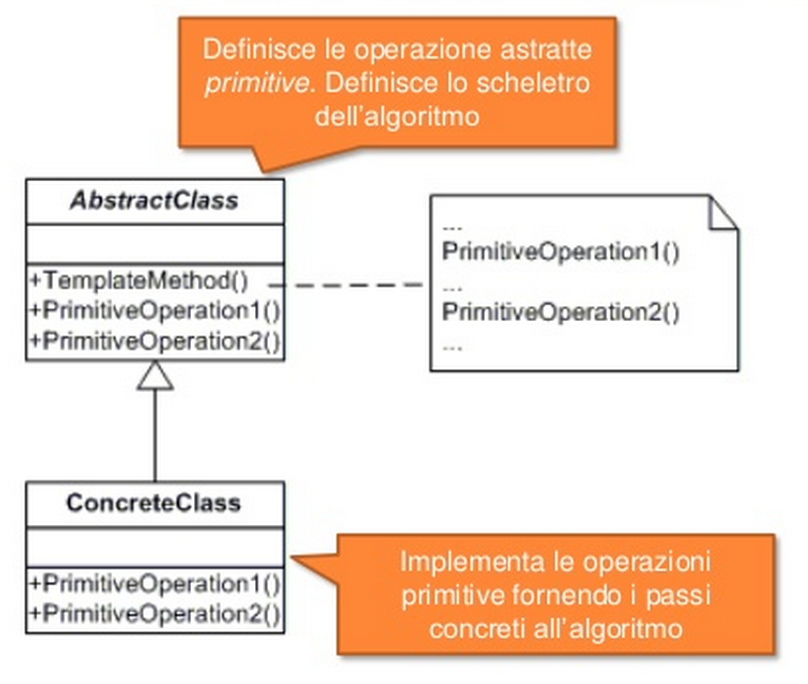
\includegraphics[width=0.8\textwidth]{immagini/templateMethod.png}
    \caption{Template method}
\end{figure}
\FloatBarrier

\subsubsection{Casi tipici}
\begin{itemize}
\item \`{E} necessaria un'unica implementazione astratta di un algoritmo;
\item Si vuole raccogliere un comportamento comune a più classi in un unica classe;
\item La classe padre deve essere in grado di eseguire i metodi delle classi figlie;
\item Tutte o quasi tutte le sottoclassi devono implementare lo stesso comportamento.
\end{itemize}